%!TEX root = foo-thesis.tex


\chapter{Implementation}
\label{chap:implementation}

\section{Used Framework and Libraries}

\begin{figure}[htbp]
  \centering
  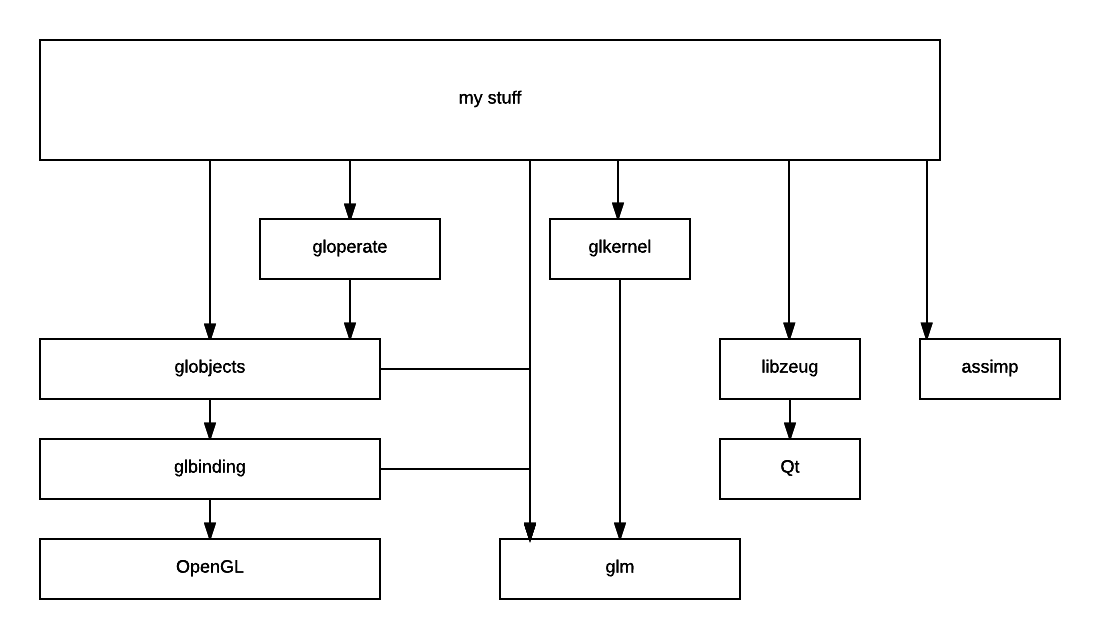
\includegraphics{graphics/Architecture}
  \caption{svg image}
\end{figure}

\begin{outline}
\1 gloperate as framework
    \2 uses qt
\1 libzeug provides GUI elements
\1 globjects as an object-oriented abstraction over OpenGL
\1 glbinding provides OpenGL bindings, directly called sometimes
\1 GLM provides math and easier interaction with the OpenGL API
\1 no further relevance for this thesis:
    \2 assimp for model loading
    \2 glkernel provides kernels for our SSAO implementation
\end{outline}

\section{Rendering Pipeline Overview}
\begin{outline}
\1 would be much the same as the concept pipeline...
\1 show what's compute shader and what not?
\1 it's basically lighting plus
    \2 g-buffer generation
    \2 shadowmap which is part of the RSM,
    \2 SSAO
    \2 deferredshading
    \2 srgb and HDR.
    \2 all of this is not
\1 model loading?
\1 kernel generation?
\end{outline}


\section{RSM Generation and VPL Sampling}
\label{sec:impl:rsmAndVplSampling}
\begin{outline}
\1 use the same code for RSM generation as for G-Buffer generation with only slight modifications:
\1 don't use normalmaps as the triangle normals are sufficient
\1 instead of individual texture lookups, we use the material's average color as diffuse color as suggested by \citet{hedman2016sequential} to avoid high-frequency color changes to affect the outcome.
\1 we re-use RSM as shadowmap
    \2 usually, one might want to decouple this since they likely need different resolutions/cascading schemes etc. One could also render the RSM with a less detailed version of the scene. Since we had no culling and LOD implemented, we were bottlenecked on geometry complexity and chose to do this in one pass.
    \2 we use variance shadowmapping. so we add the variance buffer if we're rendering an RSM, and disable another buffer (non-face normals).

\1 with a compute shader, we sample the RSM in a regular pattern and write VPLs into a buffer
\1 VPLs are position, normal, color
\1 we prepare a second buffer with a single vec4 with position in the first three values and normal packed into the last value.
\1 we do that since the ISM rendering (Section~\ref{sec:impl:ismRendering}) and light list calculation (Section~\ref{sec:impl:clusteredShading}) do not need color and especially ISM rendering reads several VPLs per point, using a lot of bandwidth.
\1 Because of the regular sampling, the noise produced during interleaved shading (Section~\ref{sec:impl:interleavedShading} or only results? there was a paper that sorts VPLs to avoid the noise...) is more structured. To help with that, we permutate the VPL order with a random permutation computed on CPU
\end{outline}


\section{ISM Rendering}
\label{sec:impl:ismRendering}

Both the point splat renderer and the single-pixel point renderer share the first stages of their rendering pipelines, which are described here, before the following subsections describe the two renderers themselves and the pull-push postprocessing.

We make use of OpenGL's tessellation shader to subdivide triangles to make them meet a certain maximum size. The tessellation control shader determines the tessellation levels according to the triangle's size. The tessellation evaluation shader does nothing more than correctly interpolating the vertex positions.

The geometry shader, which now recieves the smaller, tessellated triangles, converts the triangle to a point. The point's center equals the triangle's center, and the radius is chosen so the areas of the point and triangle match.

\todo[color=yellow]{implement that area thing}

While a random subset of all points needs to be chosen for each ISM, special care must be taken to make sure that the same subset of points is used for each ISM in each frame. Otherwise, the ISMs will be temporally incoherent and cause flickering in the final rendering. To this end, the point's barycentric coordinate inside its triangle and the triangle's primitive ID are passed to a fast hashing algorithm. The result is is used to determine an ISM ID (or, equivalently, a VPL ID) for use in the next step.

Note that no translation or projection has been applied yet, this happens in a later stage. As a result, the vertex shader is a simple pass-through shader.

The next step depends on whether point splatting or the single-pixel renderer is enabled.



\subsection{Point Rendering with Splatting}

In the case of point splatting, the geometry shader itself reads the VPL with the ID it determined, projects the point according to the VPL's data, performs culling (backface and hemisphere) sets \texttt{gl\_PointSize} to the projected size, and emits a vertex.

The \texttt{output\_primitive} must be set to \texttt{points} in the geometry shader's \texttt{layout} definition. As explained previously, for point splatting all points are simply enlarged by a small constant factor in lieu of the pull-push postprocessing. Since only depth information are needed in this case, the fragment shader is empty.



\subsection{Single-Pixel Point Rendering with Compute Shaders}

This approach was inspired by the fact that the surface reconstruction in \citet{Marroquim:2007:reconstruction} works with single-pixel ``splats''. Since in this case the hardware rasterizer is not required to achieve good performance, this allowed for more flexibility and new optimization opportunities.

The general idea is to first let the geometry shader write the generated points into a buffer, which is then used by a separate compute shader pass to perform the actual rendering.

In order to maintain temporal coherence, the points are not written into a single large buffer, as it would be hard to consistently determine a location for each point in that buffer. Instead, the buffer is divided into one section per VPL, and the points are written into the section corresponding to the ID calculated before. An atomic counter that indicates the first free index is used per section to sequentially fill these sections without overwriting any data. The order of the points within each section is undefined, but that does not change the output since they all are going to be rendered into the same ISM.

Now a compute shader is used to render the points. For each VPL, one work group reads through the respective section of the point buffer and performs the transformation and culling against the VPL for each point. It then uses \texttt{imageAtomicMin} to ``render'' the point with correct depth testing as a single pixel into the respective ISM. Since atomic operations require using single channel integer textures, it is not possible to use a second or third channel for additional attributes. Instead, the ISM is actually implemented as 3D texture, using the second index in the third dimension as additional ``render target'' to hold the radius and normal. This alse requires the attributes to be packed into a 32-bit integer.

As an optimization, the compute shader renders each point into several ISMs. To this end, each work group reads the data for a fixed number of VPLs (e.\,g.\ 16) into shared memory. Then, for each point culling is performed on all 16 VPLs, and those that pass the culling test are collected into a local array. Thereafter the point is transformed for each of the collected VPL and rendered into the respective ISM.

% In practice it turned out to be more efficient to limit the number of slots in the local array to a constant maximum (e.\,g.\ 4), possibly because this ensures that the rendering loop is not diverging and enables compiler optimizations like loop unrolling.

An attempt to do this optimization in the splat renderer by emitting multiple vertices in the geometry shader resulted in a significant performance hit, a problem not uncommon when using geometry shaders. While emitting additional vertices alone had a huge impact, the additional fillrate and overdraw became an issue when using too many points, a bottleneck that is unlikely to occur when using the single-pixel renderer.


\subsubsection{Race Conditions caused by second render target??}

There are two race conditions that may influence the output.

First, the order of writes to the ISM depth buffer is undefined as the execution order of the different compute shaders is undefined in the OpenGL specification. Therefore, the classical z-fighting may occur if two points are rendered into the same pixel of the same shadowmap with the same depth value. The attributes that end up written into the additional render target are undefined and may differ between subsequent frames. In practice, this happens very rarely and we chose to ignore this.

However, a different race condition was frequently observable in our implementation:
If two threads with differing depth values simultaneously write into the depth buffer, using \texttt{imageAtomicMin} guarantees the correct value will end up in the depth buffer. However, if the higher value got written first and gets overwritten by the second write, both writes have succeeded. This results in both threads attempting to write into the second buffer, creating another race condition since the here execution order is undefined again. THis problem can be alleviated by adding a synchronization point after the atomic write and then reading the memory location that just got written to. If it is equal to the written value, one can assume the write actually succeeded and did not get overwritten by a second, simultaneous write. Only then the write to the second buffer is performed.

However, this solution fixes the race condition only inside one work group and not between work groups, for which no efficient synchronization primitives exist on the GPU. The problem occurred infrequently enough though to be negligible.

A proper solution that would fix this problem completely, avoiding the synchronization overhead and open more optimization possibilities would involve a more advanced software renderer, e.\,g.\ following the approaches of \citet{Laine:2011:SoftwareRasterization}.


\subsection{Pull-Push Postprocessing}

Our implementation of the pull-push algorithm is relatively straightforward. For each miplevel to be calculated, one \texttt{dispatchCompute} is called. Since the first step of the pull phase has different inputs than the subsequent steps (it only has depth and size, not the displacement vector and depth interval), a slightly different shader is used there. Analogous the last step of the push phase outputs only depth, therefore a shader variant is used for that step as well. For the same reason, the input texture (the ``render target'' used by the single-pixel renderer) and output texture (the final ISM used later for shadowing) have different formats than the mipmap levels used by the pull-push algorithm.



In the pull phase, one compute shader invocation calculates one output pixel. It reads its four input pixels, determines which of them are valid, and uses the valid ones for interpolating.


During the push phase, groups of four output pixels share the same input pixels. This can be exploited by letting each shader invocation computing four output pixels while still reading only four input pixels. Naturally, the weights applied to the input pixels need to be adjusted per output pixel. For invalidating input pixels, their weights can simply be set to zero instead of separately marking them as invalid.

%Since this technique is heavily bandwidth-bound, we aggressively pack the data.
\todo[color=yellow]{actually pack this shit aggressively. 32bit depth and depth interval, 32bit displacement and radius and that's it. }

Note that there is still lots of room for optimization. Especially the pull phase is basically a parallel reduction which is well-researched and for which optimized algorithms on the GPU exist, see e.\,g.\ \citet{Harris:2007:ParallelReduction}. Several optimizations from that field might be applicable here.



\section{Interleaved Shading with Compute Shaders}
\label{sec:impl:interleavedShading}
\begin{outline}
\1 often, de-interleaving is implemented by splitting the G-buffer into several smaller G-buffers, each containing all pixels with the same sample set \cite{segovia2006non}. Each G-buffer is processed with its respective sample set, and then the buffers are re-interleaved into a large G-Buffer again.

\1 instead, we do this in a single pass. compute shaders are launched so that each invocation processes one pixel, and invocations within a work group process the same VPL set.
\1 \ref{lst:???}?
\1 diagram of the pixels. \ref{fig:impl:pixels} explain this. we still do coherent VPL processing.
\1 more explanation on id calculation
\1 reasons for single pass? 1. Easier to implement. 2. Basically, we completely remove the separate interleaving and deinterleaving step and simply change the read and write patterns, saving on the absolute amount of memory read and written. 3. Less memory used since no additional buffers are needed. 4. scales better to 8x8 interleaving pattern, since 64 interleaving sections ??? might introduce significant overhead (interleaving through buffers: maximum render targets often 8 or 16, so now multiple passes needed, interleaving through shared memory: becomes impossible, too large work groups, too much shared memory needed)
\1 potential downside is that we introduce one scattered read compared to several coherent reads in the buffer splitting method. but, bottleneck is lookups in the VPL buffer and the respective shadowmaps in the main loop, as well as ALU operations, so this one-time lookup doesn't have any impact. maybe completely latency covered or workgroups are distributed in a way that the reads are still cache-coherent.
\1 in fact, any attempts to do coherent reads did not result in speedups.

\todo[color=yellow]{investigate into interleaving via shared memory in 2x2 groups}
\todo{write hedman, how did they do the 8x8 interleaving? or maybe check his master thesis first}

\1 Since only a subset of all samples is processed per pixel and this subset repeats every four pixels, this process results in structured noise (see Figure \ref{fig:???} or this figure in concept?)
\1 therefore, geometry-aware blur similar to \citet{laine2007incremental}. doesn't smooth over edges. two passes for vertical and horizontal. See code snippet \ref{listing:???}.

\1 VPL shuffling helps a great deal! See Figure \ref{fig:impl:shuffling}
\end{outline}

\section{Clustered Deferred Shading}
\label{sec:impl:clusteredShading}

\begin{outline}
\1 we use 128 pixels as screen-space tile width and 16 depth slices. We also use an optimization proposed by \citet{persson::2013::practical} and use a larger near cluster for better depth slice utilization.

\1 \citet{persson::2013::practical} do culling on the CPU. they have small radii and can therefore quickly determine the clusters that are reached by a certain light.
\1 we have infinite light radii and therefore lots of clusters per light. therefore, we can expect to cull maybe half the lights and not the majority.
\1 therefore, we decided to iterate over all lights per used cluster, as opposed to iterate over reached clusters per light.
\1 the more uniform control flow of this approach as also better suited to GPUs.


\1 three phases, each corresponding to one dispatch compute call:
\1 clustering
    \2 each work group processes one tile and has one 16 bool array which indicates which depth slices in that tile are used.
    \2 for each fragment, set the corresponding bool to true. no synchronization needed.
    \2 since the work group size is limited, we set it to 128 and let each invocation iterate through 128 pixels in the tile to cover all pixels.
    \2 per work group, count the number of used slices
        \3 we use the first 16 threads in the work group and atomic adds, but one could just as well let one thread do it serially, it doesn't matter.
    \2 then it adds the number of used depth slices to one global atomic counter. the glsl function to do this returns the value of the counter before the addition.
    \2 this way, each workgroup ``allocates'' some space in the list of used clusters. it then writes an id for each cluster into that list.
\1 calculating light lists
    \2 one invocation per used cluster.
    \2 calculate world-space corners of that cluster.
    \2 show some code? but it's really ugly...
    \2 for each light
        \3 if any corner is inside the illuminated hemisphere, add the light to this cluster's light list.
    \2 we simply allocate the maximum space for this.
        \3 for full HD / 128\,px tiles = 135 tiles, * 16 depth slices = 2160 light lists, * 1024 vpls = 2160k indices, * 2 bytes per index makes 4mb.
        \3 we thought it's unnecessary to cut that down.
        \3 by a (conservative) estimate of four used depth slices per tile on average, (plus possibly runtime checks to allocate more space when running over that limit), on could reduce this to 1MB with little implementation effort.
        \3 compacting the light lists themselves is probably not worth it due to implementation complexity and performance penalty
        \3 since we expect to cull roughly half the lights, the potential saving by compacting the light lists is only 50\% anyways.
\1 shading
    \2 during shading, when processing a pixel, the pixel's cluster is first determined and only the lights of this cluster's light list are processed.
    \2 we use a very basic approach to combine this with interleaved shading: of all lights in the light list, each pixels gets an equally sized fraction. while this might lead to adjacent pixels processing overlapping sets of lights if they are in different clusters, they are either in clusters near to each other in which case the light lists are probably quite similar, or they are in clusters seperated from each other so the geometry-aware blur wouldn't consider them anyway.

\1 Tiled shading
    \2 In addition to clustered deferred shading, we also implemented its predecessor tiled shading. Since it does not perform a clustering in the z-dimension and thus has only one cluster per tile, it allows for a simpler implementation.
    \2 We integrated this directly into our final gathering shader. Since each work group processes all pixels that are in the same tile and use the same set of VPLs for lighting, we can easily do the following:
        \3 each invocation reads one pixel. With six shared variables (minimum and maximum x, y and z values) and the atomicMin and atomicMax methods, create an exact bounding box in NDC
        \3 now, each invocation takes one VPL and culls it against the bounding box. If it passes the culling test, it adds it to a list in shared memory, again using an atomic counter that describes the list's current size to not overwrite any VPL added by another invocation.
        \3 perform the regular final gathering, using the list of VPLs in shared memory.

\todo[]{remove all we}

\todo[color=yellow]{rename gi shader to final gathering. other renames?}
\todo{what openGL version do i require? also, i should look up which dedicated GPUs support 4.5/4.4 and what Intels GPUs say. maybe point out the need for modern OpenGL more? also, how they make it easier to implement.}
\end{outline}

\todo[color=blue]{textify implementation}
